\chapter{Introduction}
\textbf{Adarsh Pyarelal}

\section{Purpose and structure}

This document serves the following purposes.

\begin{itemize}
    \item Declare the capabilities we aim to demonstrate for our online agent
        components in ASIST Study 3
    \item Declare in advance -- with as much specificity as we can muster --
        the offline analyses we plan to perform on ASIST study 3 data.
\end{itemize}


The goal of the preregistration process as originally devised
\citep{Nosek.ea:2018} is to separate hypothesis-generating (exploratory)
research from hypothesis-testing (confirmatory) research. A large portion of
the activities engaged in by TA1 performers in ASIST - e.g., development of
models, algorithms, and systems - does not fit neatly into the paradigm of
hypothesis generation and testing.  For this reason, while we endeavor to
specify our analyses and capabilities in as much detail as we can, we do not
specify specific social science style hypotheses to be tested\footnote{Whether
TA1 performers \emph{should} be specifying formal, quantitative hypotheses is
another discussion.}.

One of the primary motivations for this preregistration document from the
perspective of a TA1 performer team is to accelerate the writing up of
manuscripts for publication by using the structure provided by the
preregistration process to plan ahead for publications.

Each of the sections in this document is a `component preregistation' that
corresponds to a publication `seedling', with the content optimized for what we
call `copy-pasteability', that is, the ability to be copied verbatim into a
manuscript for publication with minimal changes. This is intended to reduce
duplicate effort between writing up preregistrations and publications.

Since we are a fairly large team, each section has the names of the primary
authors responsible for the content of the section displayed under the section
heading. Authorship is ascribed to those who have contributed substantially to
the ideation or writing of the content.

\section{Overview}

Broadly speaking, we are aiming to develop a suite of open-source technologies
for artificial social intelligence, with a focus on computational understanding
of spoken team dialogue. Each of the component preregistrations demonstrates a
capability that we believe is important for artificial social intelligence, and
is currently integrated or will be integrated in the near future into our ASI
agent that will be evaluated in ASIST study 3 or future ASIST experiments.

\begin{itemize}
    \item Describe the architecture of the ToMCAT ASI and ACs. Provide one or
        more architecture diagrams.
    \item Give a brief summary of the preregistrations and how they contribute
        to the overall architecture.
\end{itemize}

\begin{figure}
    \centering
    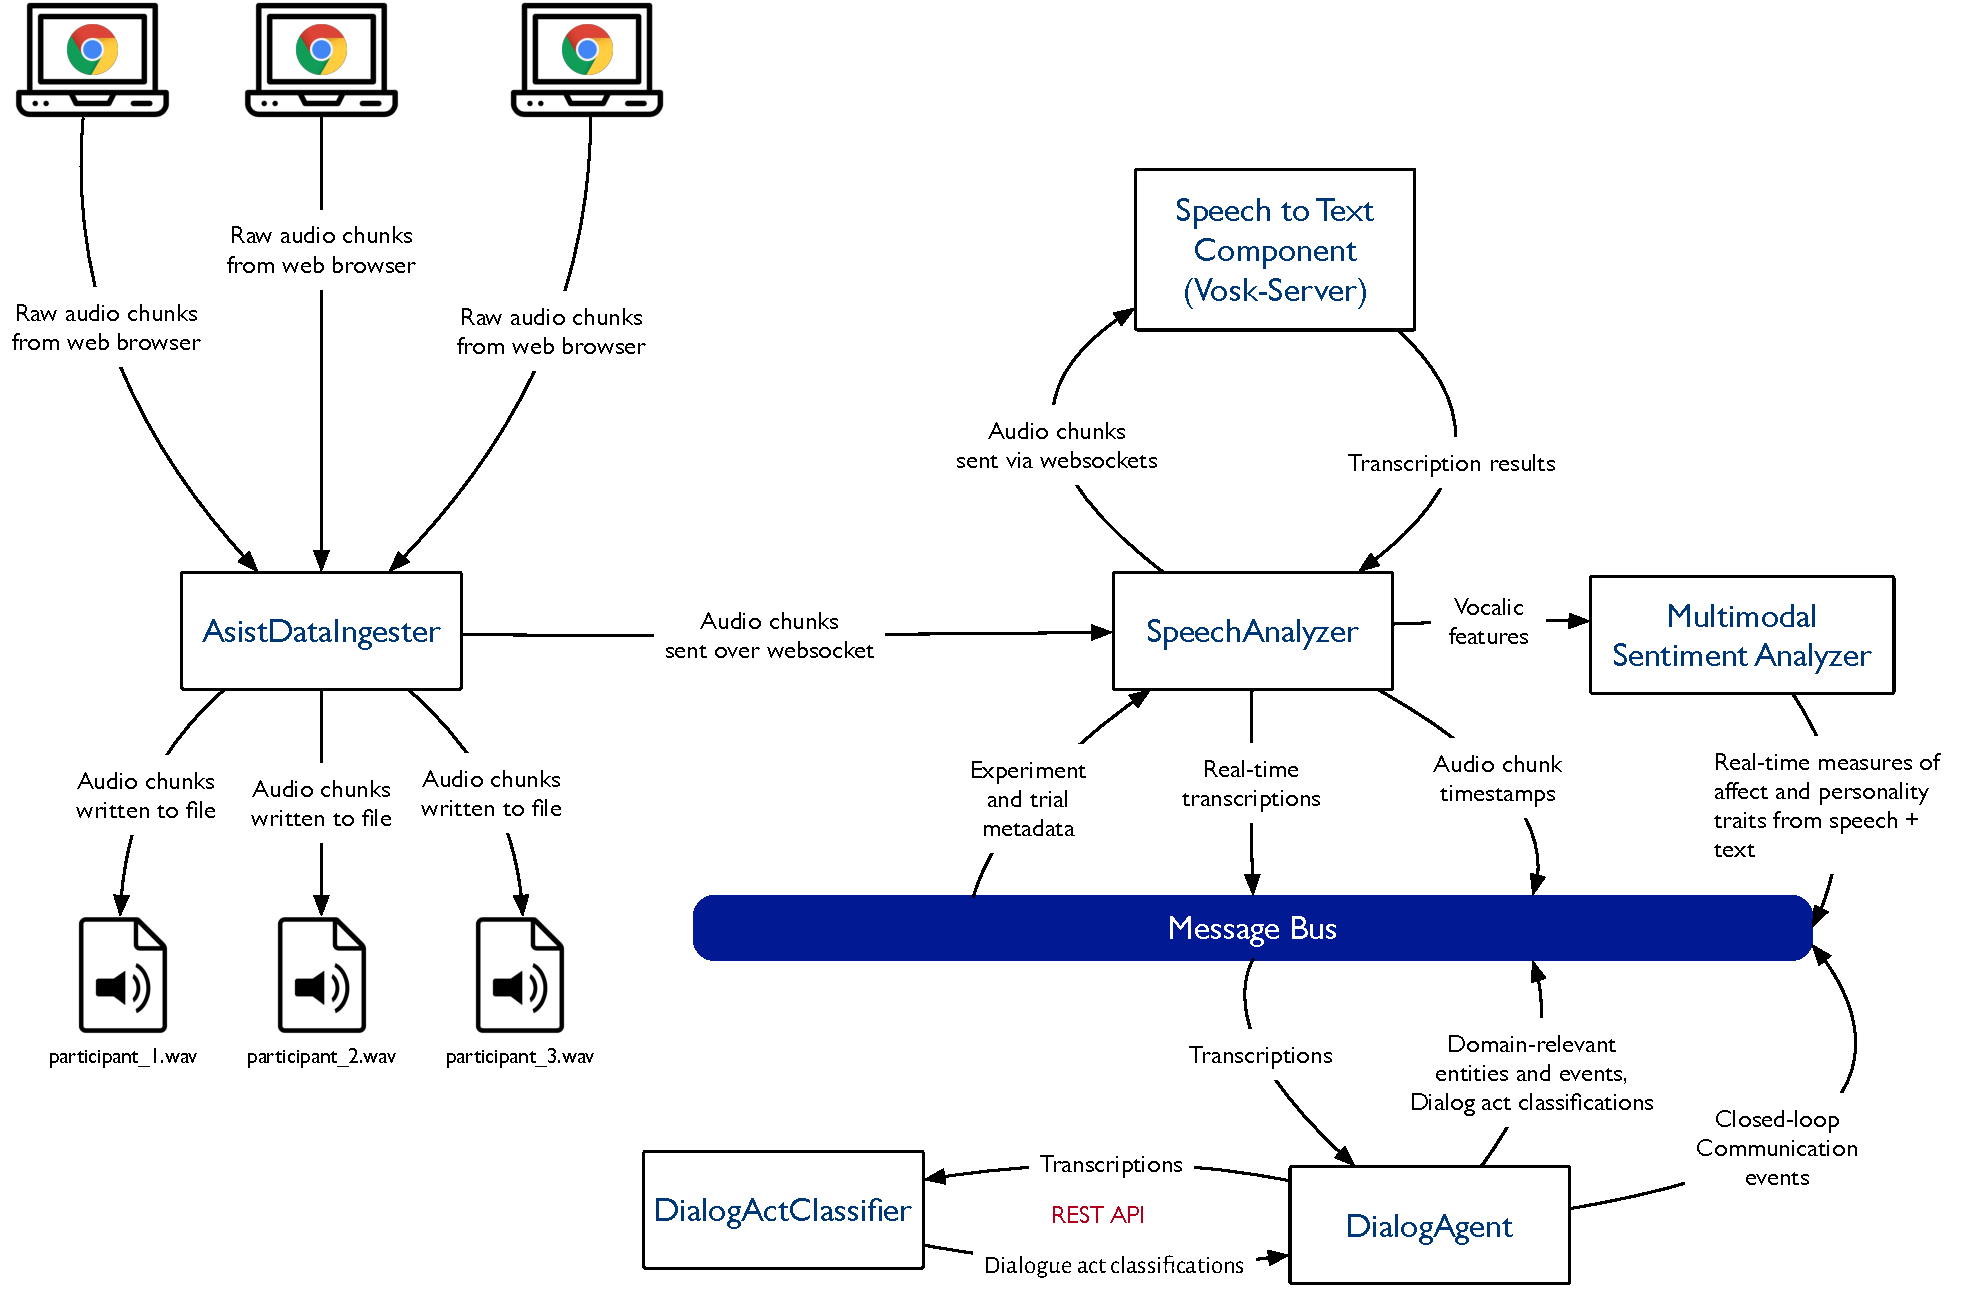
\includegraphics[width=6.5in]{images/nlp_architecture}
    \caption{Architecture of our multi-participant dialogue analysis system.}
\end{figure}

